
%%%%%%%%%%%%%%%%%%%%%%% file typeinst.tex %%%%%%%%%%%%%%%%%%%%%%%%%
%
% This is the LaTeX source for the instructions to authors using
% the LaTeX document class 'llncs.cls' for contributions to
% the Lecture Notes in Computer Sciences series.
% http://www.springer.com/lncs       Springer Heidelberg 2006/05/04
%
% It may be used as a template for your own input - copy it
% to a new file with a new name and use it as the basis
% for your article.
%
% NB: the document class 'llncs' has its own and detailed documentation, see
% ftp://ftp.springer.de/data/pubftp/pub/tex/latex/llncs/latex2e/llncsdoc.pdf
%
%%%%%%%%%%%%%%%%%%%%%%%%%%%%%%%%%%%%%%%%%%%%%%%%%%%%%%%%%%%%%%%%%%%


\documentclass[runningheads,a4paper]{llncs}
\usepackage{graphicx}
\usepackage{url}
\usepackage[listings]{tcolorbox}
\usepackage{amssymb}
\usepackage{pifont}

\newcommand{\critics}{{\small{\sc{Critics}}}}
\newcommand{\phabricator}{{\small{\sc{Phabricator}}}}
\newcommand{\gerrit}{{\small{\sc{Gerrit}}}}
\newcommand{\codeflow}{{\small{\sc{CodeFlow}}}}
\newcommand{\collaborator}{{\small{\sc{Collaborator}}}}
\newcommand{\clusterchanges}{{\small{\sc{ClusterChanges}}}}
\newcommand{\delCode}{\textcolor{black}}
\newcommand{\addCode}{\textcolor{black}}
\newcommand{\ttt}[1]{\tt\small{#1}}


% -----------------------------------------------------------------
% color
% -----------------------------------------------------------------
\definecolor{javared}{rgb}{0.6,0,0} % for strings
\definecolor{javagreen}{rgb}{0.25,0.5,0.35} % comments
\definecolor{javapurple}{rgb}{0.5,0,0.35} % keywords
\definecolor{javadocblue}{rgb}{0.25,0.35,0.75} % javadoc

% ===============================================
% MyJavaSmallStyle
% ===============================================
\lstdefinestyle{MyJavaSmallStyle} {
  language=Java,
  frame=none,
  xleftmargin=15pt, 
  stepnumber=1, 
  numbers=left, 
  numbersep=5pt,
  numberstyle=\tiny\color[gray]{0.777}, 
  belowcaptionskip=\bigskipamount,
  captionpos=b, 
  escapeinside={*'}{'*},
  tabsize=5,
  emphstyle={\bf},
  basicstyle=\scriptsize\ttfamily,
  keywordstyle=\color{javapurple}\bfseries,
  stringstyle=\color{javared},
  commentstyle=\color{javagreen},
  morecomment=[s][\color{javadocblue}]{/**}{*/},
  showspaces=false,
  columns=flexible,
  showstringspaces=false,
  morecomment=[l]{//},
  tabsize=2,
  morekeywords={, Package,Invariant,Class,Method,Field,Where,in,Assert,ToLc,Split,Msg,Immutable,<<<,eq,neq,not,has,Assert,AssertExists,Attribute,Uc,Lc,},
  breaklines=true
}

\usepackage{amssymb}
\setcounter{tocdepth}{3}

\usepackage{url}
\usepackage{booktabs}
\usepackage{amsmath} 

\newcommand{\keywords}[1]{\par\addvspace\baselineskip

\noindent\keywordname\enspace\ignorespaces#1}
\newcommand{\codefont}[1]{\footnotesize{\texttt{#1}}\normalsize}

\begin{document}

\mainmatter  % start of an individual contribution

% first the title is needed
\title{Software Evolution} 

\author{Na Meng, Tianyi Zhang, Miryung Kim} 

\institute{Virginia Tech and University of California, Los Angeles} 
\toctitle{Handbook on Software Engineering} 
\tocauthor{Na Meng, Tianyi Zhang and Miryung Kim}
\maketitle


\begin{abstract}
	\todo{Miryung is in charge.} 
\end{abstract}


\section{Introduction}
\todo{2 page-Miryung is in charge}
- explain the definition of software evolution (cite: belady and lehman, etc)
%L.A. Belady and M.M. Lehman, a Model of Large Program Development,o IBM Systems J., vol. 15, no. 1, pp. 225±252, 1976.
\cite{Belady1976:ModelEvolution} 
% follow up work by Yuen 
@inproceedings{ChongHokYuen1986:EAS,
 author = {Chong Hok Yuen, C S},
 title = {An Empirical Approach to the Study of Errors in Large Software Under Maintenance},
 booktitle = {The Institute of Electrical and Electronics Engineers, Inc on Conference on Software Maintenance--1985},
 year = {1985},
 isbn = {0-8186-0648-7},
 location = {Washington, D.C, USA},
 pages = {96--105},
 numpages = {10},
 url = {http://dl.acm.org/citation.cfm?id=20924.20936},
 acmid = {20936},
 publisher = {IEEE Press},
 address = {Piscataway, NJ, USA},
} 

% some overview materials can be drawn from then introduction of kemerer paper. 
- describe why this chapter focus on code changes, rather than other types of artefacts such as requirements, specifications, design documents, etc. 
- argue why software evolution is important (cite: code decay, eick et al.) 
\cite{Eick2001:CodeDecay}

\section{Concepts and Principles}
\label{sec:concepts}

In this section, we focus on software changes---an important aspect of software evolution. To that end, we will first introduce the categorization of software changes, and then overview three principled ways of dealing with software changes. These concepts and principles will navigate our tour of seminal papers in the next section.

\subsection{Classifying Software Changes}
Swanson initially identified three categories of software changes: corrective, adaptive, and perfective~\cite{Swanson1976:Dimension}. These categories were updated later and ISO/IEC 14764 instead presents four types of changes: corrective, adaptive, perfective, and preventive~\cite{iso}.
\subsubsection{Corrective Change} refers software modifications initiated by software defects. A defect can result from design errors, logic errors, and coding errors~\cite{Longstreet1990:smc}.

\begin{itemize}
\item Design errors: software design does not fully align with the requirement specification. The faulty design leads to a software system that either incompletely or incorrectly implements the requested computational functionalities. 
\item Logic errors: a program behaves abnormally by terminating unexpectedly or producing wrong outputs. The abnormal behaviors are mainly due to flaws in software functionality implementations.
\item Coding errors: although a program can function well, it takes excessively high runtime or memory overhead before responding to user requests. Such failures may be caused by loose coding, or the absence of ``reasonableness checks'' on computations performed.
\end{itemize}

\subsubsection{Adaptive Change} is a change introduced to accommodate any modifications in the environment of a software product. The term \textbf{environment} here refers to the totality of all conditions that influence the software product, including business rules, government policies, and software and hardware operating systems. For example, when porting a mobile application from Android to iOS, mobile developers need to apply adaptive changes to translate the code from Java to Swift, so that the software is still compilable and executable on the new platform. Programs may be also changed as a result of a new compiler, which performs additional optimizations to generate smaller and faster code. 

%when maintaining a legacy system that was written in Fortran decades ago, programmers may migrate the system to a mainstream general purpose language, such as Java, to facilitate the maintenance of existing codebase and to extend the system by leveraging new features of the popular language. When building phone apps, Mobile developers may port a mobile application from one platform (e.g., Android) to another (e.g. iOS) by translating code from Java to Swift. 
\subsubsection{Perfective Change} is the change undertaken to expand the existing requirements of a system~\cite{Seaman2008:SMC}. When a software product becomes useful, users always expect to use it in new scenarios beyond the scope for which it was initially developed. Such requirement expansion causes changes to either enhance existing system functionalities or add new features. For instance, an image processing system was originally developed to process JPEG files, and later experienced a series of perfective changes to also handle other formats of images, such as PNG and SVG.

\subsubsection{Preventive Change} is the change applied to prevent malfunctions or to improve maintainability of software. 
According to Lehman's laws of software evolution~\cite{Lehman1984:ULE}, the long-term effect of corrective, adaptive, and perfective changes is deteriorating the software structure while increasing entropy. Preventive changes are usually applied to address the problems. For instance, after developers fix some bugs and implement new features in an existing software product, the complexity of source code can increase to an unmanageable level. Through code refactoring---a series of behavior-preserving changes, developers can reduce the code complexity, and increase both readability and reusability of the software.

\begin{figure}[!htb]
\centering
\scalebox{0.6}{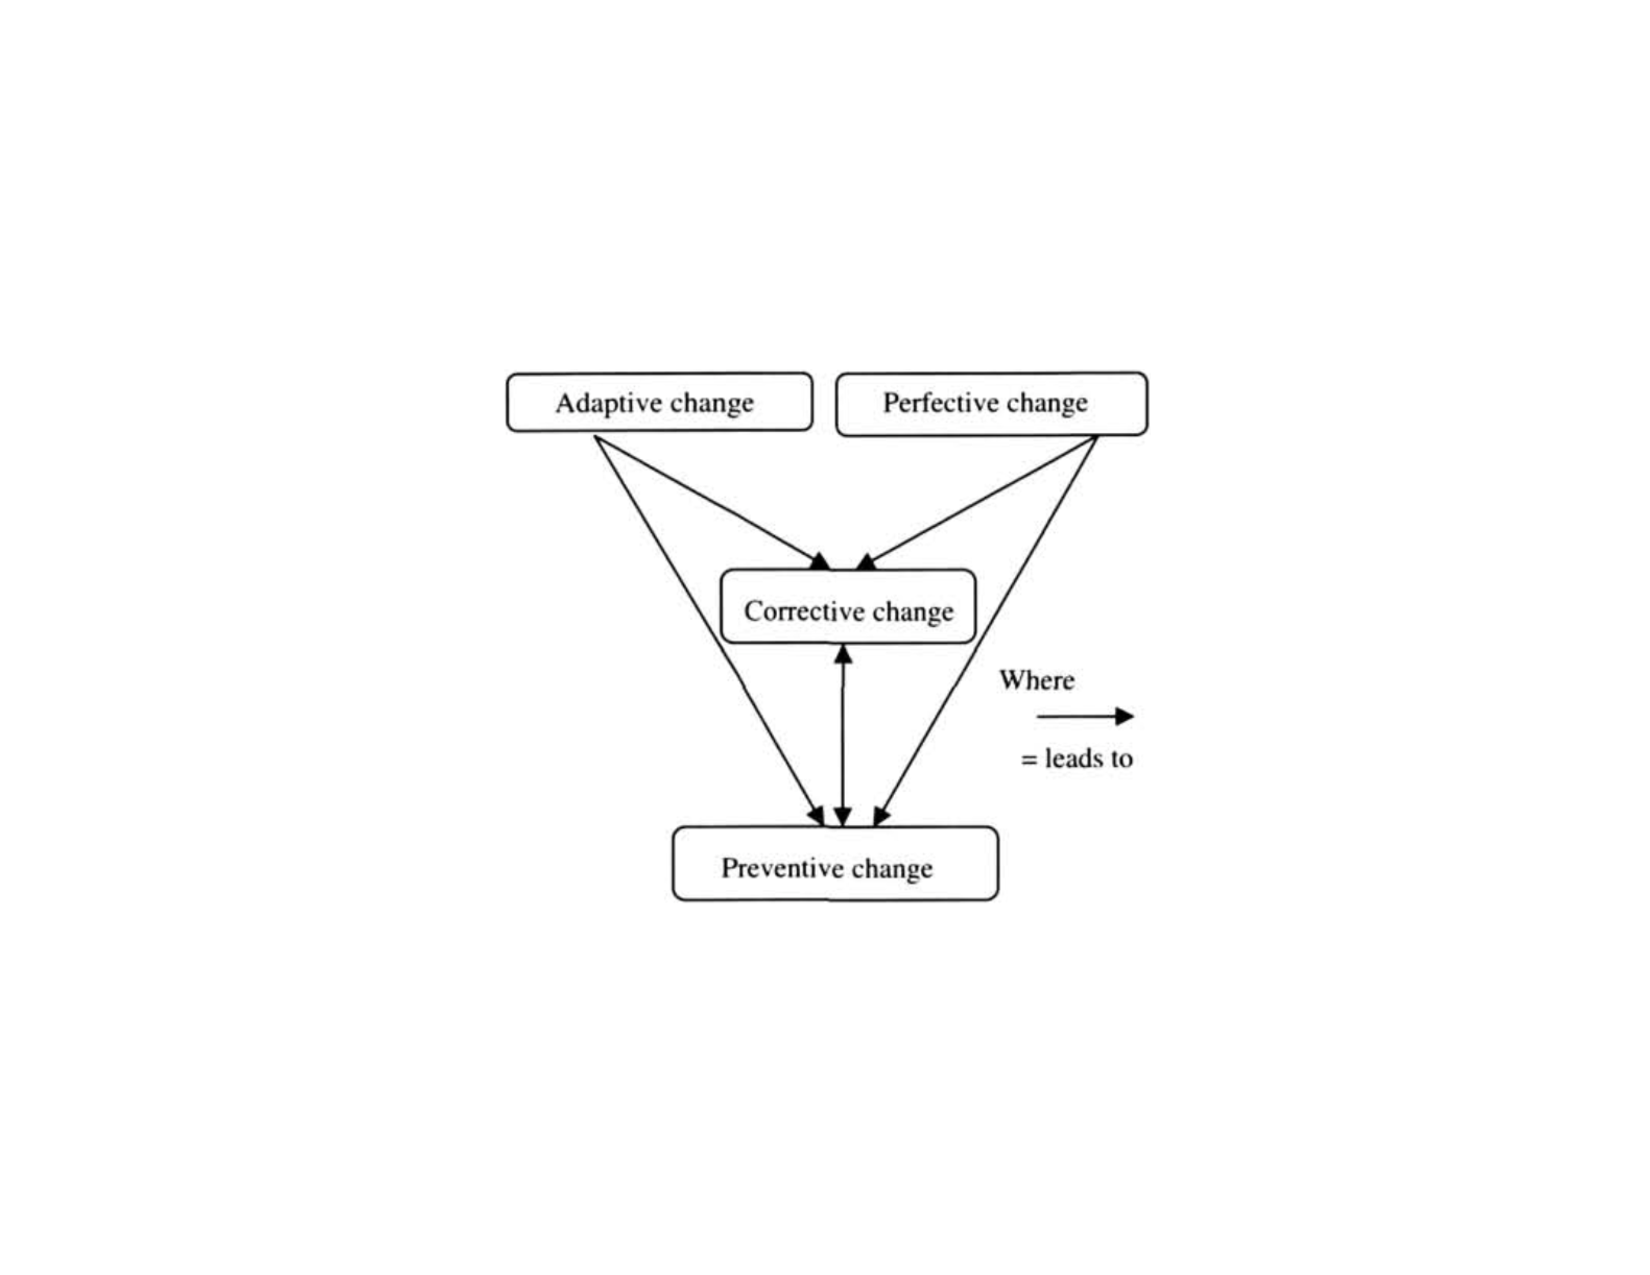
\includegraphics{images/relationship_of_changes.pdf}}
\caption{Potential relation between software changes~\cite{Seaman2008:SMC}}
\label{fig:relation}
\end{figure}

Figure~\ref{fig:relation} presents the potential relationships between different types of changes~\cite{Seaman2008:SMC}. Specifically, both adaptive changes and perfective changes may lead to the other two types of changes, because developers may introduce bugs or worsen code structures when adapting software to new environments or implementing new features. Preventive changes may be led to by all the other three kinds of changes, corresponding to the Lehman's laws mentioned above.

\subsection{Handling Software Changes}

When evolving software, developers may apply various kinds of changes either manually or with some tool support. There are mainly two principled ways frequently used to check the correctness of applied changes. First, programmers other than the change creator perform code reviews based on their understanding of the program, and provide feedback if they capture any suspicious software modification. Second, developers and testers create or reuse test cases based on the requirements specification, run the modified program against the test cases, and check whether the software executes as expected.  

In the following three sections, we will discuss the seminal papers focusing on the above-mentioned three principled ways to deal with software changes: applying changes (Section~\ref{sec:apply}), inspecting changes (Section~\ref{sec:inspect}), and debugging and testing changes (Section~\ref{sec:debugtest}).  

\section{An Organized Tour of Seminal Papers: I. Applying Program Changes}
\label{sec:apply}
In Section~\ref{sec:corrective}-\ref{sec:preventive}, we will discuss research topics separately relevant to the four types of software changes mentioned in Section~\ref{sec:concepts}. Next, we will introduce automatic change application regardless of the change types  in Section~\ref{sec:automatic}.

\subsection{Corrective Change}
\label{sec:corrective}
Corrective changes, or software bug fixes, are frequently applied by developers to eliminate defects in software. There are mainly two lines of research conducted: empirical studies to characterize bugs or their fixes~\cite{Fenton2000:QAF,Li2006:TCE,Kim2006:MBF,Lu2008:LMC,Nguyen2010:RBF,Yin2011:FBB,Park2012:supplementary,Zhong2015:ESR}, and automatic approaches to help developers detect and fix bugs~\cite{Engler2000:CSR,Bush2000:SAF,Hangal2002:TDS,Hovemeyer2004:FBE,Naik2006:ESR,Weimer2009:AFP}. There is no clear boundary between the two lines of research, because some prior work~\cite{Li2006:CPMiner,Pham2010:DRS,Jin2012:UDR,Kim2013:PAR} did leverage the characteristics observed in empirical studies to automatically detect and fix bugs.

\subsubsection{Characterization Studies of Bug or Fixes}
To analyze bug characteristics, Li et al.~conducted an empirical study on bugs from two popular open source projects: Mozilla and Apache HTTP Server~\cite{Li2006:TCE}. By manually examining 264 bug reports from the Mozilla Bugzilla database~\cite{mozilla}, and 209 bug reports from the Apache Bugzilla database~\cite{asf}, they investigated the root cause, impact, and software components of each software error that exhibited abnormal runtime behaviors. They observed three major root causes: memory, concurrency, and semantics. The memory bugs account for 16.3\% in Mozilla and 12.2\% in Apache. Among memory bugs, NULL pointer dereference was observed as a major cause, accounting for 37.2-41.7\%. More importantly, semantic bugs were observed to be dominant, accounting for 81.1\% in Mozilla and 86.7\% in Apache. One possible reason is that most semantic bugs are specific to applications. A developer can easily introduce semantic bugs while coding, due to a lack of thorough understanding of the software. It is challenging to automatically detect or fix such bugs, because diagnosing and resolving them require a lot of domain-specific knowledge.

To characterize bug fixes, Kim et al.~conducted an empirical study on bug fixing data from the change history of five open source projects: ArgoUML, Columba, Eclipse, jEdit, and Scarab~\cite{Kim2006:MBF}. With keywords like ``Fixed'' or ``Bugs'', they retrieved code commits in software version history that are relevant to bug fixes, chopped each commit into contiguous code change blocks (i.e., hunks), and then clustered similar code changes. They observed that 19.3-40.3\% bugs appeared repeatedly in version history, while 7.9-15.5\% of bug-and-fix pairs appeared more than once. The results demonstrate that project-specific bug fix patterns occur frequently enough to be useful as a bug detection technique. Furthermore, for the bug-and-fix pairs, it is possible to both detect the bug and provide a strong suggestion for the fix. 

\begin{table}[]
\centering
\caption{Sample system rule templates and examples from~\cite{Engler2000:CSR}}
\label{tab:rule}
\begin{tabular}{l|l}
\toprule
Rule template                  & Example                                                 \\ \hline
``Never/always do X''          & ``Do not use floating point in the kernel''             \\\hline
``Do X rather than Y''         & ``Use memory mapped I/O rather than copying''           \\ \hline
``Always do X before/after Y'' & ``Check user pointers before using them in the kernel''\\
\bottomrule
\end{tabular}
\end{table} 

\subsubsection{Automatic Bug Detection and Fixing Approaches} 
Engler et al.~defined a meta-language for users to easily specify temporal system rules such as ``release locks after acquiring them''~\cite{Engler2000:CSR}. They also extended a compiler to interpret the rules and dynamically generate additional checks in the compiler. If any code snippet violates the specified rule(s), the approach reports the snippet as a software bug. Table~\ref{tab:rule} presents some exemplar system rule templates and instances. 
With this approach, developers can flexibly define their own rules to avoid some project-specific bugs, without worrying how to implement checkers to enforce the rules.

Li et al. developed CP-Miner, an automatic approach to find copy-paste related bugs in large-scale software~\cite{Li2006:CPMiner}. CP-Miner was created based on a prior empirical study~\cite{Chou2001:ESO}, which revealed that under the Linux {\sf drivers/i2o} directory, 34 out of 35 errors were caused by copy-paste or duplicated code. 
One of the major reasons why copy-paste introduces bugs is that when developers copy code from one location and paste it to another location, they forget to consistently rename identifiers of variables, functions, and types. CP-Miner first identifies copy-paste code in a scalable way, and then detects bugs associated with copy-paste by checking the renamed identifiers. If an identifier is inconsistently renamed, with some of its occurrences replaced and some not replaced, CP-Miner reports it as a copy-paste bug. Many previously unknown bugs in popular operating systems were detected in this way, 49 in Linux and 31 in FreeBSD, meaning that CP-Miner can effectively capture copy-paste related bugs. 
 
\subsection{Adaptive Change}
\label{sec:adaptive}
Adaptive changes are applied to a software product when its environment changes. In this section, we focus on two scenarios when adaptive changes are applied: software library upgrade and cross-language software migration.

\subsubsection{Software Library Upgrade} 
When building new software (e.g., a search engine), instead of coding everything from scratch, developers always extend existing frameworks or third-party libraries (e.g., Lucene~\cite{lucene}) by invoking the Application Programming Interfaces (APIs), to reuse the well implemented and fully tested functionalities. However, as library developers release new versions of their software to fix existing bugs and include new features, client developers should also upgrade the libraries used in their projects to benefit from the newer versions. Ideally, the library APIs should be stable so that such software upgrades do not incur any program change in client applications. In reality, nevertheless, these APIs are susceptible to changes, requiring client developers to apply adaptive changes for the usage of new library versions. 

\begin{figure}
\centering
\scalebox{0.4}{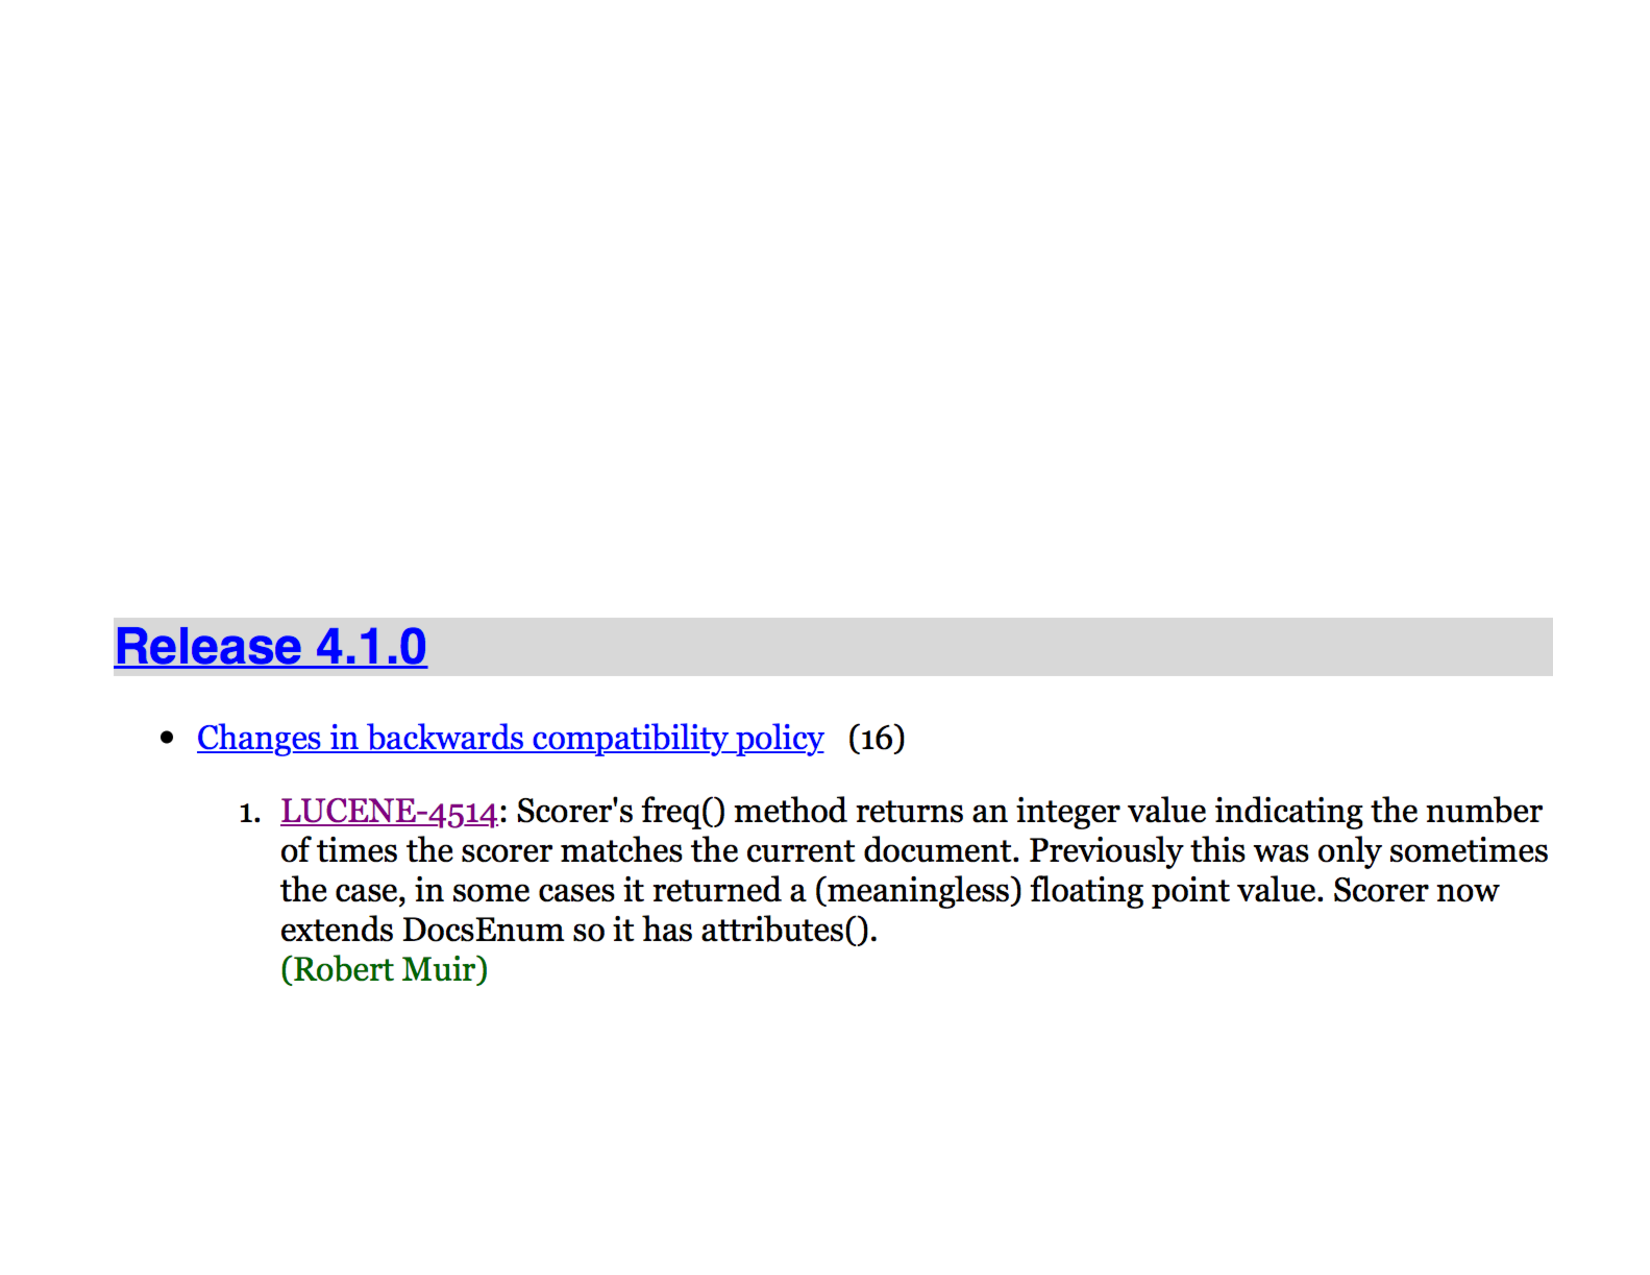
\includegraphics{images/releasenote.pdf}}
\caption{An excerpt of the Lucene change log for Release 4.1.0~\cite{releasenote}}
\label{fig:releasenote}
\end{figure}

Figure~\ref{fig:releasenote} presents an excerpt of the Lucene change log for Release 4.1.0~\cite{releasenote}. According to the release note, there are 16 recent changes in the library that can make client applications incompatible with the new release, requiring client developers to manually resolve the issues. Among the 16 changes, the first one is about a return type change of Scorer's \codefont{freq()} method. Previously, the method returns a float number, and now it returns an integer. Correspondingly, client code should be changed to properly process the new values returned by this method. By manually checking such release notes and searching for candidate solutions online, client developers can apply adaptive changes to solve any incompatibility issue between client code and new library releases.

Researchers have proposed approaches to automatically infer and recommend such adaptive changes for framework or library evolution~\cite{Dagenais2008:RAC,Schafer2008:MFU,Zhong2009:MMR,Wu2010:AHA,Nguyen2010:GAA}. For instance, Dagenais et al.~developed SemDiff, an automatic approach that compares two releases of a library or framework to infer any adaptive change of API replacements~\cite{Dagenais2008:RAC}. Suppose in the old library release, there are two methods: \codefont{caller1} and \codefont{caller2}, both of which invoke a library public API \codefont{m1()}. However, in the new library release, both methods instead invoke another public API \codefont{m2()}. Therefore, SemDiff infers an API replacement pattern \codefont{m1()->m2()}. When scanning a client application built on the old library release, SemDiff automatically recommends the inferred adaptive change for every invocation of \codefont{m1()}.

\subsubsection{Cross-language Software Translation}
When maintaining a legacy system that was written in an old programming language (e.g., Fortran) decades ago, programmers may migrate the system to a mainstream general-purpose language, such as Java, to facilitate the maintenance of existing codebase and to extend the system by leveraging new features of the popular language. Different from the API adaptive changes mentioned above, such software translation requires of a significant amount of coding effort to rewrite the same application in a new programming language.

TXL is a source transformation language designed to translate or manipulate programming languages~\cite{Cordy2006}. As shown in Figure~\ref{fig:txl}, a typical TXL file consists of two parts. The first part defines a context-free grammar to describe program syntax, while the second part describes a set of transformation rules to manipulate the syntax. For our illustrative example, the grammar defines a simple language that only allows numbers, addition and subtraction numerical expressions. The rule \codefont{resolveAddition} describes the resolution of an addition expression by replacing the expression with a number value \codefont{N1 [ + N2 ]}. Given such a file, the TXL program transformation engine automatically transforms programs of the syntactic structure by applying the rules. 
%However, manually defining translation rules using this domain-specific language is still cumbersome and error-prone for developers.

\begin{figure}
\centering
\scalebox{0.5}{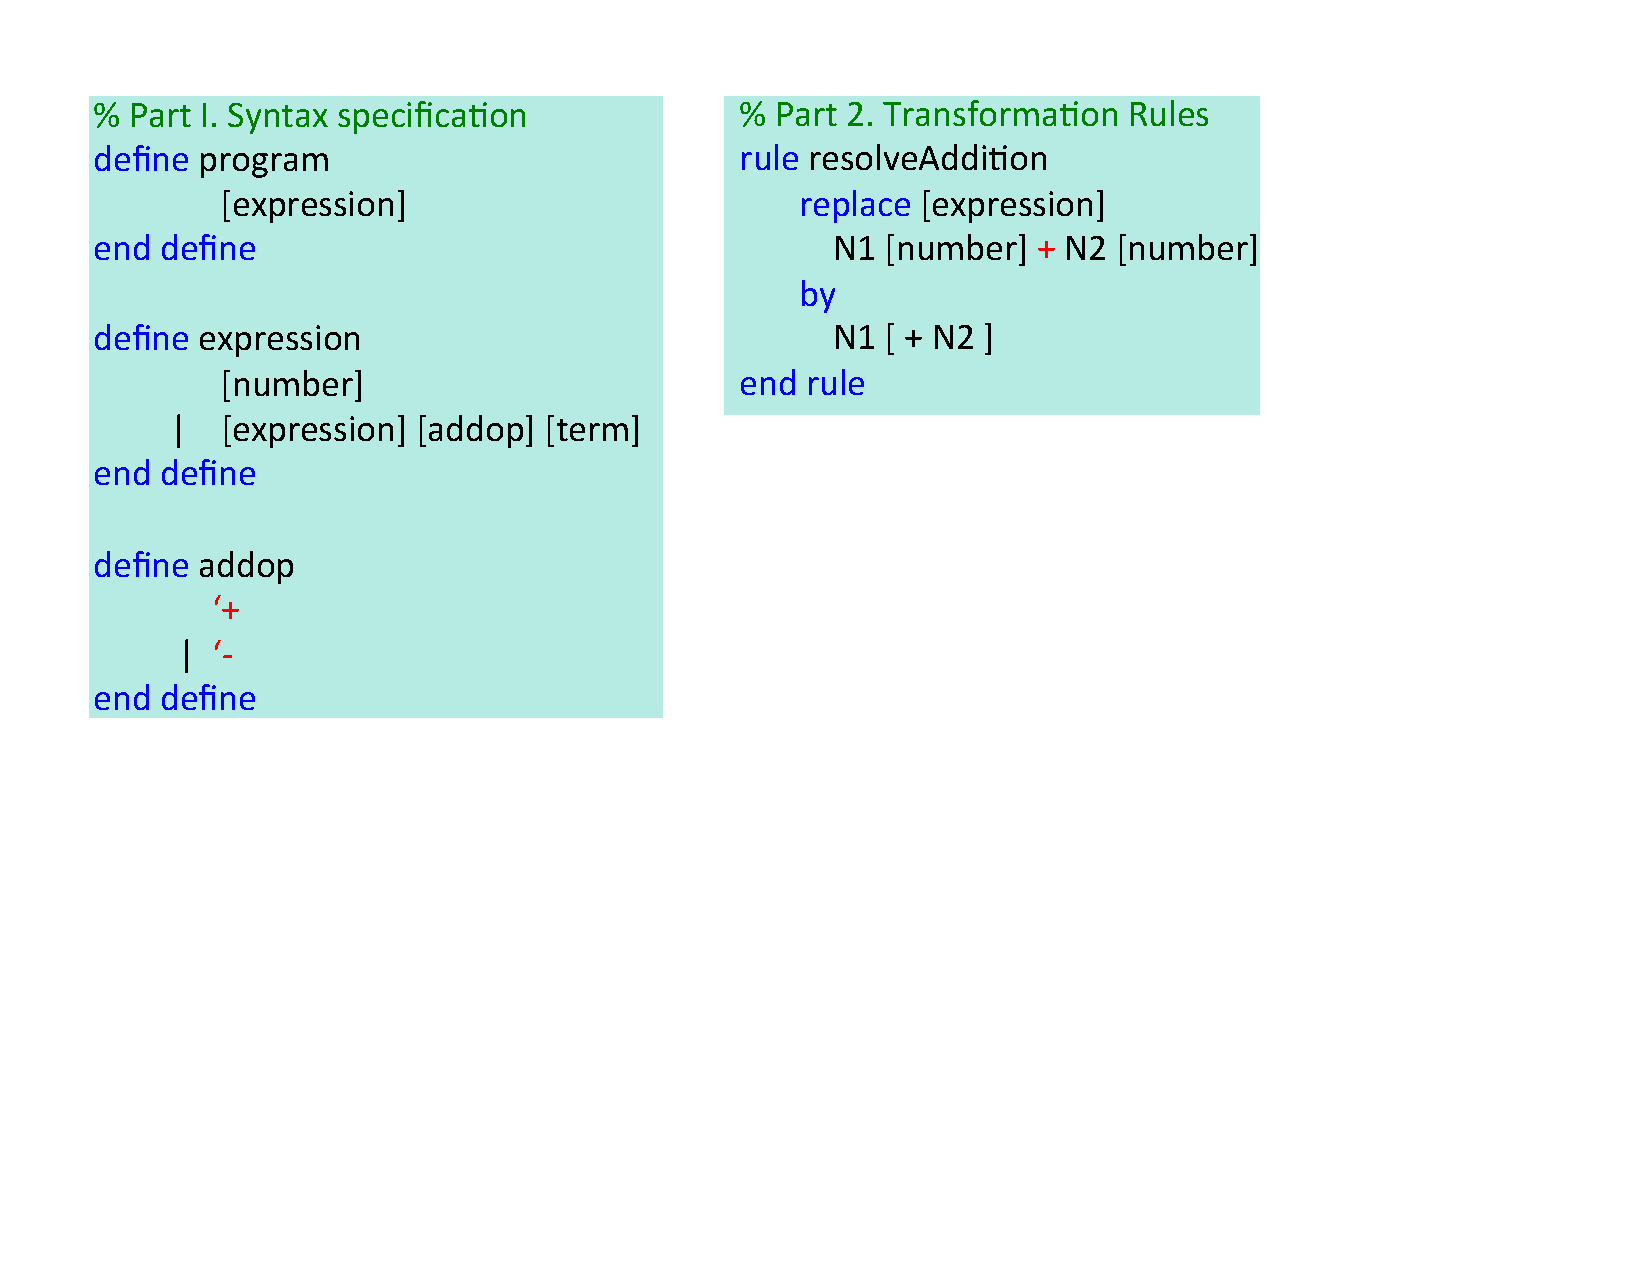
\includegraphics{images/txl.pdf}}
\caption{A simple exemplar TXL file based on~\cite{txltour}}
\label{fig:txl}
\end{figure}
With TXL, developers to not need to build programming language translators by coding every line of implementation. Instead, the transformation engine can automatically translate code once developers specify all needed grammars and rules. Researchers built tools using TXL to automate various code translation tasks, like ASP-to-NSP and Java-to-C\#~\cite{Chu:08,Hassan:2005,El-Ramly:2006,Tonella:04}.
%For instance, Hassan et al. migrated web applications between different web development frameworks like ASP and NSP~\cite{Hassan:2005}, while El-Ramly et al.~converted Java programs to C\#~\cite{El-Ramly:2006}. 

\subsection{Perfective Change}
\label{sec:perfective}
Developers apply perfective changes when enhancing or adding software features by implementing new code. There is not much research done in this area to facilitate feature enhancement or addition. One possible reason is that the implementation logic is always project-specific and spontaneous. It is challenging for any automatic tool to predict what new code to add, and to suggest what rules to apply when integrating new code with existing codebases. In this section, we mainly focus on two most closely relevant research topics: Aspect Oriented Programming (AOP) and Feature Oriented Programming (FOP).

\subsubsection{AOP} is a programming paradigm that aims to increase modularity by allowing the separation of cross-cutting concerns~\cite{Kiczales1997}. Suppose developers want to add a new feature---logging---to log all executed functions. 
The logging logic is straightforward: printing the function's name at each function's entry. However, manually inserting the same implementation to each function body is tedious and error-prone. With AOP, developers only need to first define the logging logic as \textbf{an advice}, and then specify the place where to insert the advice (i.e., \textbf{pointcut}), such as the entry point of each function. An aspect weaver will read the aspect-oriented code, and generate appropriate object-oriented code with the aspects integrated. In this way, AOP facilitate developers to efficiently introduce new program behaviors without cluttering the core implementation in the existing codebase. Many Java bytecode manipulation frameworks implement the AOP paradigm, like ASM~\cite{asm}, Javassist~\cite{javassist}, and AspectJ~\cite{aspectj}, so that developers can easily modify program runtime behaviors without touching the source code. 


\subsubsection{FOP} is a paradigm for program generation in software product lines and for incremental development of programs~\cite{Batory1992:DIH}. 
FOP is closely related to AOP. Both deal with modules that encapsulate crosscuts of classes, and both express program extensions.
In FOP, every software is considered as a composition of multiple features or layers. Each feature implements a certain program functionality, while features may interact with each other to collaboratively provides a larger functionality or get adapted to each other.
A software product line (SPL) is a family of programs where each program is defined by a unique composition of features. Formally, FOP considers programs as \emph{values} and program extensions as \emph{functions}~\cite{Lammel2013:fop}. Suppose there are two programs: 

$f \text{	// program with feature }f$, and

$g\text{	// program with feature }g$.

\noindent
A program extension is a function that takes a program as input and produces a feature-augmented program output. Suppose there are two program extensions:

$i \bullet x$ // adds feature i to program x, and 

$j \bullet y$ // adds feature j to program y.

By applying the functions to the values, we can compose more than one multi-featured application as below:

$app1 = i \bullet f$ // app1 has features i and f,

$app2 = j \bullet g$ // app2 has features j and g, and
 
$app3 = i \bullet j \bullet f$ // app3 has features i, j, f.

\subsection{Preventive Change}
\label{sec:preventive}
Program refactorings~\cite{Fowler1999:refactoring} are usually conducted to increase software maintainability, readability, or reliability, and to prevent problems in future. Fowler et al.~introduced 71 code refactorings that developers can apply to their code, and summarized why and how to apply each refactoring~\cite{Fowler1999:refactoring}. Typically, a refactoring process consists of the following activities~\cite{Mens2004:SSR}:
\begin{enumerate}
\item Identifying where to apply what refactoring(s).
\item Checking that the refactoring to apply preserves program behaviors.
\item Refactoring the code.
\item Assessing the effect of applied refactoring on software quality (e.g., complexity and readability). 
\item Maintaining the consistency between refactored code and other related software artifacts, like documentation, tests, and issue tracking records.  
\end{enumerate}

Researchers have proposed different approaches, techniques, or formalisms to support each of above activities.

\subsubsection{Identifying Where to Apply What Refactorings}
Various approaches have been proposed to automatically suggest refactoring opportunities based on program context, code smell, or version history~\cite{Balazinska2000:ACA,Kataoka2001:ASP,Higo2008:metricrefactoring,Tsantalis2011:rankRefactoring,Wang2014:recommendClones,Meng2015:ARO}. Specifically, Kataoka et al.~developed Daikon to infer program invariants at runtime, and thus suggest candidate refactorings~\cite{Kataoka2001:ASP}. For instance, if Daikon observes that one parameter of a method is always constant, it then suggests a \emph{removeParameter} refactoring. Balazinska et al.~used a clone detection tool to identify duplicated code and to suggest clone removal refactorings~\cite{Balazinska2000:ACA}. Tsantalis et al.~ranked clones that have been repetitively or simultaneously changed in the past to suggest refactorings~\cite{Tsantalis2011:rankRefactoring}. Wang et al.~extracted features from code to reflect program context, code smell, and evolution history, and then used a machine learning technique to rank clones for refactorings~\cite{Wang2014:recommendClones}.

\subsubsection{Checking the Behavior-Preserving Property of Refactorings}
A refactoring is behavior-preserving, if given the same set of input values, a program always produces the same set of output values before and after the refactoring~\cite{Opdyke1992:ROF}. Opdyke suggested to ensure such behavior preservation by specifying \emph{refactoring preconditions}~\cite{Opdyke1992:ROF}. For instance, when conducting an \emph{create\_method\_function} refactoring, before inserting a member function $F$ to a class $C$, developers should specify and check for five preconditions, as shown in Figure~\ref{fig:preconditions}. If any precondition is not satisfied, the refactoring should not be applied.

\begin{figure}[!htb]
\centering
\scalebox{0.55}{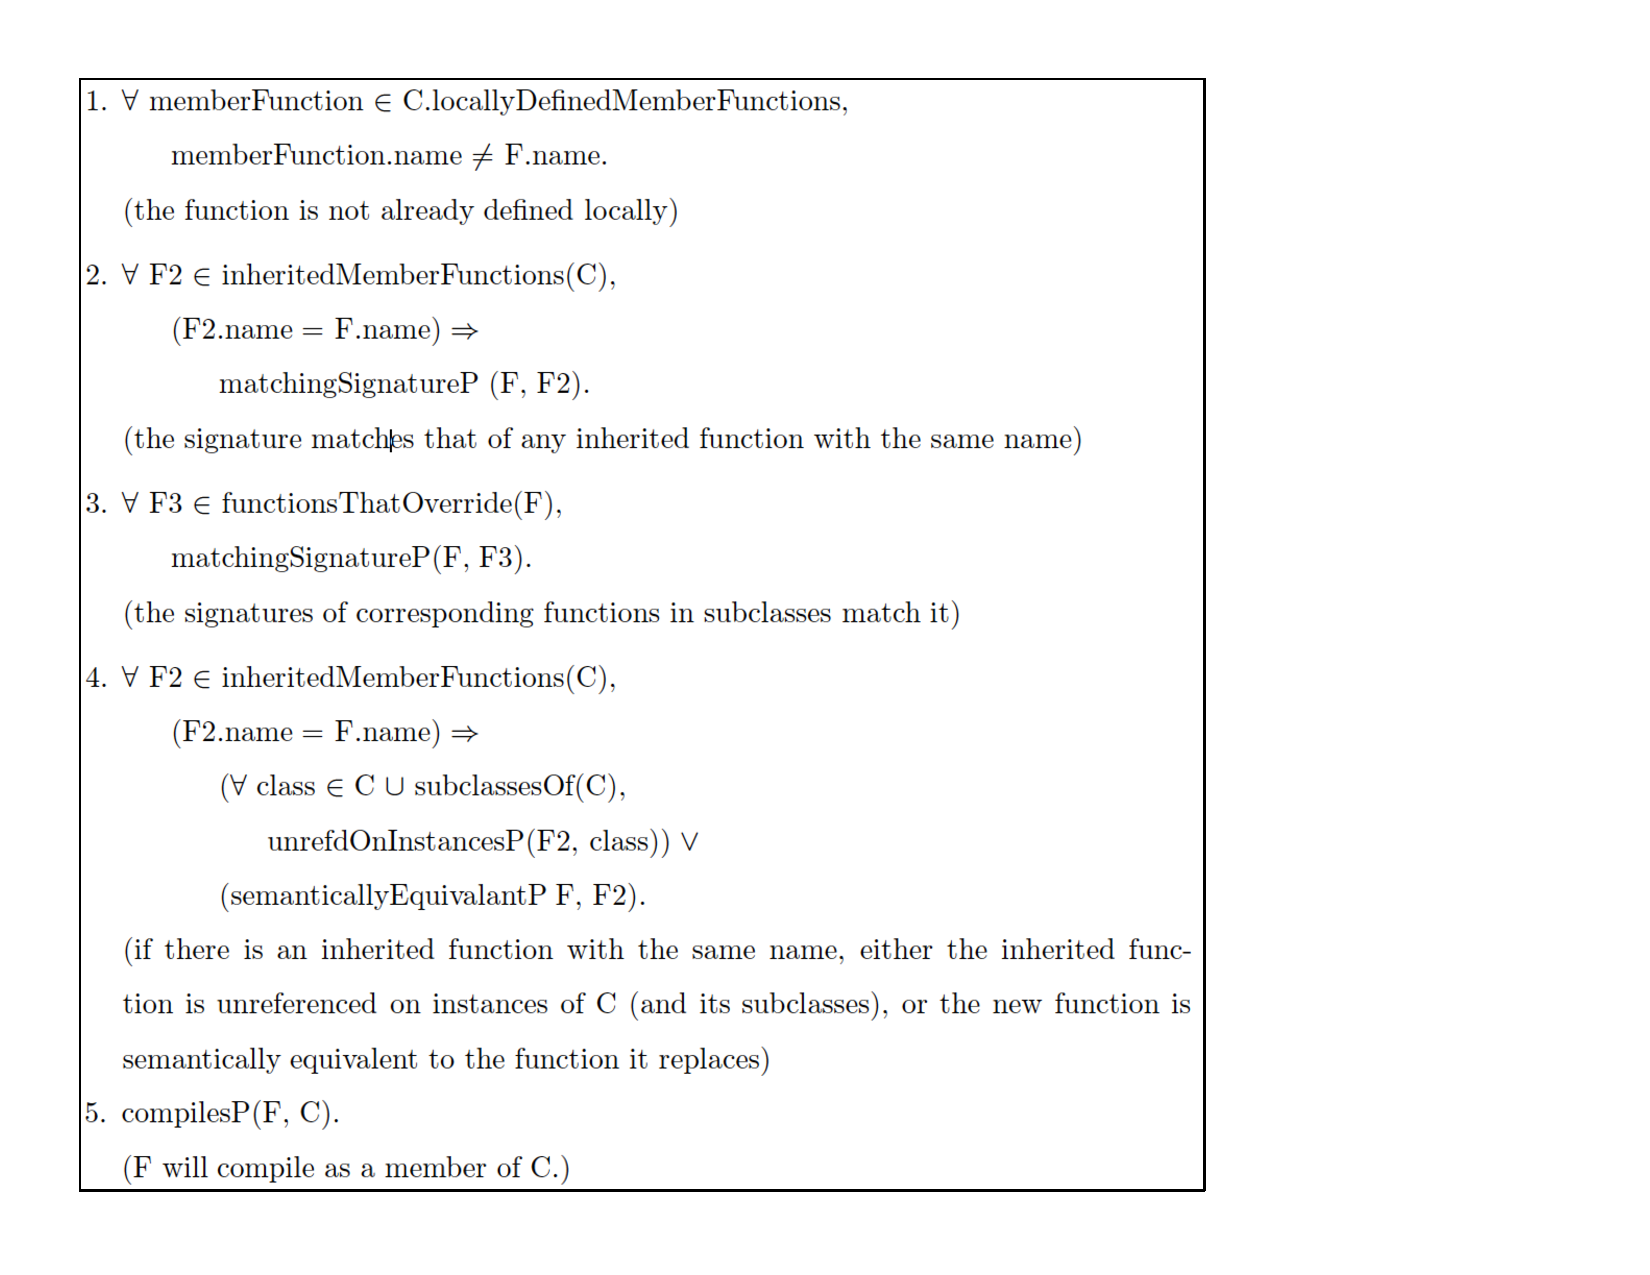
\includegraphics{images/preconditions.pdf}}
\caption{Preconditions for the \emph{create\_method\_function} refactoring~\cite{Opdyke1992:ROF}}
\label{fig:preconditions}
\end{figure}

\subsubsection{Applying Refactorings}
The Eclipse IDE provides automatic support for a variety of refactorings, including \emph{rename}, \emph{move}, and \emph{extractMethod}. With such support, developers do not need to worry about how to check preconditions or postconditions before manually applying a certain refactoring. Instead, they can simply select the refactoring command from a menu (e.g., \emph{extractMethod}), and provide necessary information to accomplish the refactoring (e.g., method name). The Eclipse refactoring engine takes care of the precondition check, program transformation, and postcondition check. Additionally, 
researchers conducted empirical studies to characterize the refactorings applied by developers~\cite{Kim2012:FSR,Murphy-Hill2012:refactor,Vailian2012:misuse,Silva2016:WWR}, and proposed various approaches to automate refactoring or to complete the refactoring tasks initiated by developers~\cite{Griswold:1992,Balazinska1999,Dig:2009,Ge:2012,Chen:2013,Lee:2013,Tsantalis2013:icsm,Meng:2015,Kim:2016}. For instance, Silva et al.~observed that refactoring activity is mainly driven by changes in the requirements and much less by code smells~\cite{Silva2016:WWR}. Kim et al.~developed R3, an alternative refactoring engine that works 10 times faster than Eclipse Refactoring~\cite{Kim:2016}. 

\subsubsection{Assessing the Effect of Refactoring} 
To understand whether any refactoring application actually improves software quality, researchers proposed 
different techniques to measure the impact of refactorings~\cite{Kataoka2002:evaluateRefactor,Tahvildari2003:MAE}. Specifically, Kataoka et al.~proposed coupling metrics to evaluate the refactoring effect~\cite{Kataoka2002:evaluateRefactor}. By comparing the coupling before and after the refactoring, they assessed the degree of maintainability enhancement. Similarly, Tahvildari et al.~suggested using a catalogue of object-oriented metrics to estimate refactoring impact, including complexity metrics, coupling metrics, and cohesion metrics~\cite{Tahvildari2003:MAE}. 
 
\subsubsection{Maintaining Consistency of Refactored Software} 
Approaches were investigated to ensure the consistency between refactored programs and other software artifacts like design models~\cite{Bottoni2003:coordinatedTransformation,Straeten2003:UML}. For example, Bottoni et al.~modeled a refactoring as a set of distributed graph transformations~\cite{Bottoni2003:coordinatedTransformation}. Each time a code refactoring is applied, the corresponding graph transformations are automatically applied to related design models to preserve consistency. Van Der Straeten et al.~suggested using description logic to maintain the consistency between relevant UML models as they evolve~\cite{Straeten2003:UML}.
\subsection{Automatic Change Application}
\label{sec:automatic}

Various approaches were proposed to automatically suggest program changes to developers or help developers edit code, regardless of the change type. In this section, we mainly focus on Programming by Demonstration (PbD), simultaneous editing, and systematic editing.

\subsubsection{PbD} is also called Programming by Example (PbE). It is an end-user development technique for teaching a computer or a robot new behaviors by demonstrating the task to transfer directly instead of manually programming the task.
Approaches were built to generate programs based on the text-editing actions demonstrated or text change examples provided by users~\cite{Nix1984,WiM1993,LaH1995,LWD2001}. For instance, 
TELS records editing actions, such as search-and-replace, and generalizes them into a program that transforms input to output~\cite{WiM1993}. It leverages heuristics to match actions against each other to detect any loop in the user-demonstrated program. 
Similarly, SMARTedit~\cite{LWD2001} automates repetitive text-editing tasks by learning programs to perform them using techniques drawn from machine learning. SMARTedit represents a text-editing program as a series of functions that alter the state of the text editor (i.e., the contents of the file, or the cursor position). Like macro recording systems, SMARTedit learns the program by observing a user performing her task. However, unlike macro recorders, SMARTedit examines the context in which the user's actions are performed and learns programs that work correctly in new contexts. 

\subsubsection{Simultaneous Editing} repetitively applies source code changes that are interactively demonstrated by users~\cite{MiM2001}. When users apply their edits in one program context, the tool replicates the \emph{exact lexical} edits to other code fragments, or transforms code accordingly. For instance, Linked Editing requires users to first specify the similar code snippets which they want to modify in the same way~\cite{TBG2004}. As users interactively edit one of these snippets, Linked Editing simultaneously applies the identical edits to other snippets. 
CloneTracker takes the output of a clone detector as input and creates a descriptor for each clone~\cite{DuR2007}. With such descriptors, CloneTracker tracks clones across program versions and identifies any modification to those clones. 
Similar to Linked Editing, CloneTracker also echoes edits in one clone to other counterparts upon a developer's request. 
Clever is another clone management system that tracks code clone groups and detects any inconsistent change applied to clones within the same group~\cite{NNP2009}. If a clone misses the updates applied to the other clones in the same group, Clever automatically suggests the missing update to that clone.

\subsubsection{Systematic Editing} is the process of applying similar, but not necessarily identical, program changes to multiple code locations. 
%Prior work shows that programmers apply systematic edits to either add features, fix bugs, or refactor code~\cite{Kim:2005,Kim:2009,Nguyen:2010}. 
Manually applying systematic edits is tedious and error-prone. 
%for two reasons. 
%First, developers may forget to apply systematic edits to all program contexts where the edits are needed, committing errors of omission. Second, developers may apply edits inconsistently and thus introduce new bugs. 
%To improve programmer productivity and software quality, 
Several approaches~\cite{MKM2011,MKM2013,Rolim:2017} have been proposed to infer the general program transformation from one or more code change examples provided by developers, and then apply the transformation to other program contexts in need of similar changes. Specifically, LASE requires developers to provide multiple similarly changed Java methods (at least two)~\cite{MKM2013}. By extracting the commonality between demonstrated changes and abstracting the changes in terms of identifier usage and control- or data-dependency constraints in edit contexts, LASE creates a general program transformation, which can both detect code locations that should be changed similarly, and suggest customized code changes for each candidate location.

\section{An Organized Tour of Seminal Papers: II. Inspecting Program Changes}
\label{sec:inspect}

\section{An Organized Tour of Seminal Papers: III. Debugging and Testing Program Changes}
\label{sec:debugtest}



\section{Future Directions and Open Problems} 
\todo {4 pages} 


\subsubsection*{Acknowledgments.} The heading should be treated as a
subsubsection heading and should not be assigned a number.

\section{The References Section}\label{references}
\bibliography{tianyi,mengna}
\bibliographystyle{abbrv}

\section*{Appendix} 

\end{document}
